\subsection{CluStream}

\textit{CluStream} is a method developed in the Watson Research Center at IBM and the University of Illinois, UIUC. This method presented a different approach on the matter of clustering streams of data with respect to a modified version of \textit{K-Means} which was adapted to work also with data streams. The main difference relies on the separation of the clustering process into two parts: one which would handle the data stream itself gathering only statistically relevant information (online part) and another which actually process the results of the former to produce the actual clusters wanted (offline part). 

Separating the clustering process provides the user several advantages, among others:

\begin{itemize}
 \item by saving only statistical data, rather than the original content, it is possible to save physical storage space (e.g. hard drive space) and therefore reducing costs and allowing a wider range in time to be clustered.
 
 \item The method also allows the analysis of the evolution of the data, as the necessary information for that is contained in the stored statistical information.
 
 \item Because the two parts operate independently it allows the user to select a time horizon, or even a time window, to perform the offline clustering part using the stored statistical information.
\end{itemize}

\subsubsection{The CluStream framework}

This method is built over a few ideas that need to be conceptualized, which will answer fundamental questions and set up a basis of terminology useful along this work.

\begin{itemize}
 \item \textbf{Micro-Clusters}: that is the given name for the statistical information summaries that is computed during the online component. They are a temporal extension of \textit{cluster feature vectors}\cite{zhang96birch}, which benefit from an additive feature that makes them a natural choice for the data stream problem\cite{clustreamOrig}.
 
 \item \textbf{Pyramidal time frame}: micro-clusters are stored periodically following a pyramidal pattern. This allows a nice tradeoff between the ability to store large amounts of information while giving the user the possible to work with different time horizons without loosing too much precision. The statistical summaries stored are used by the offline component to compute finally the macro-clusters which are the actual clusters the user intended to get.
\end{itemize}

It is assumed that a data stream comes in the form of multi-dimensional records $\bar X_1 ... \bar X_k ...$ where $\bar X_i = (x^1_i ... x^d_i)$.

\begin{definition}\cite{clustreamOrig}

A micro-cluster for a set of d-dimensional points $X_{i_1} ...X_{i_n}$ with time stamps
$T_{i_1} ...T_{i_n}$ is defined as the $2 \cdot d + 3)$ tuple $(\overline{CF2^x},\overline{CF1^x},CF2^t,CF1^t,n)$, wherein $\overline{CF2^x}$ and $\overline{CF1^x}$ each correspond to a vector of d entries. The definition of each of these entries is as follows: 

\begin{itemize}
 \item For each dimension, the sum of the squares of the data values is maintained in $\overline{CF2^x}$. Thus, $\overline{CF2^x}$ contains d values. The p-th entry of $\overline{CF2^x}$ is equal to $\sum^n_{j=1} (x^p_{i_j})^2$. 
 \item For each dimension, the sum of the data values is maintained in $\overline{CF1^x}$. Thus, $\overline{CF1^x}$ contains d values. The p-th entry of $\overline{CF1^x}$ is equal to $\sum^n_{j=1} x^p_{i_j}$.
 \item The sum of the squares of the time stamps $T_{i_1} ...T_{i_n}$ is maintained in $CF2^t$.
 \item The sum of the time stamps $T_{i_1} ...T_{i_n}$ is maintained in $CF1^t$.
 \item The number of data points is maintained in n.
\end{itemize}

\end{definition}

\subsubsection{Maintaining the micro-clusters}

Whenever a new point arrives, it is necessary to find its nearest micro-cluster. It is possible to calculate an average radious or \textit{RMSD}, only to then compare the distance to the point to a factor of it: when the distance between a point and its nearest micro-cluster is smaller or equal to the average radiuos (of the micro-cluster in question) times a user defined factor, then this point is added to the micro-cluster. Adding a point to a micro-cluster means that the properties of the micro-cluster change, such as RMSD and size (number of points).

Whenever a point (outlier) does not fulfill the mentioned condition, then a new micro-cluster has to be created in order to give this point a chance as a potential new cluster. In order to do so, an older micro-cluster has to be deleted or two micro-clusters have to be merged. To determine which solution is appropriate a recency value for each micro-cluster has to be determined\footnote{See \cite{clustreamOrig} for more details.} and until all the micro-clusters which have an older recency value than a user specified parameter are deleted, it is possible to start merging the micro-clusters which are closest to one another.

\subsubsection{Offline macro-clusterig}

The macro-clustering part is done by selecting a time window and then performing a modified version of \textit{K-Means} to cluster the center of the current micro-clusters using the size as weights. 

Selecting a time window implies using two snapshots to determine what happened in such time window: the most recent snapshot is used as the base and the older one is used to determine overlapping micro-clusters. Once this is determined, a simple sustraction of their properties is performed to obtain the correct set of micro-clusters to use in the macro-clustering step.

\subsection{SPARK}
\textit{Apache Spark} is an open source framework developed in the AMPLab at the University of California, campus Berkeley\cite{SparkResearch}. It is a fast and general engine for large-scale data processing, as they describe it themselves. The original goal was to design a new programming model that supports a wider class of applications than MapReduce and at the same time keeping the fault tolerance property of it. They claim MapReduce is inefficient for applications that require a multi-pass implementation and a low latency data sharing across parallel operations, which are common in data analytics nowadays, such as: 

\begin{itemize}
 \item Iterative algorithms: many machine learning and graph algorithms.
 \item Interactive data mining: multiple queries on data loaded into RAM.
 \item Streaming applications: some require an aggregate sate over time.
\end{itemize}

Traditionally, MapReduce and DAG engines are based on an acyclic data flow, which makes them non optimal for these applications listed above. In this flow, data has to be read from a stable storage system, like a distributed file system, and then processed on a series of jobs only to be written back to the stable storage. This process of reading and writing data on each step of the workflow causes a significant rise in computational cost.

The solution proposed offers \textit{resilient distributed datasets (RDDs)} to overcome this issue efficiently. RDDs are stored in memory between queries (no need of replication) and they can rebuild themselves in case of failure as they remember how they were originally built from other datasets by transformations such as \textit{map, group, join}.

\subsection{SPARK streaming}

For this project, Spark streaming plays an important role as it takes a raw data stream and transforms it so that it is possible to process it within the framework. A raw stream of data can come in different forms and through different channels: from a very simple file stream, where whenever a new file is added to a specific location it is recognized as the input, a socket stream where the data comes through the network using a TCP protocol and also integrates with more elaborated sources such as \textit{Kafka, Flume, Twitter, HDFS/S3,} etc.


\begin{figure}[h!]
 \centering
 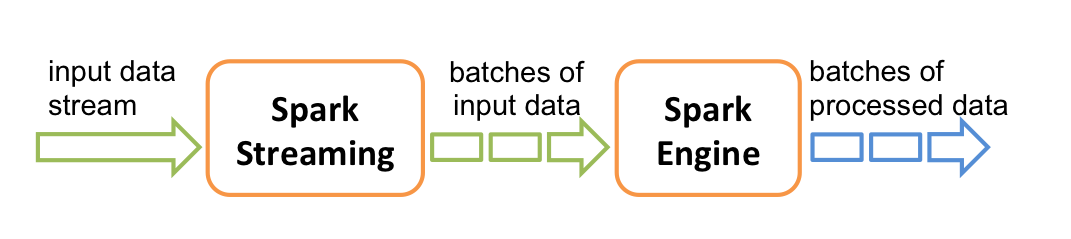
\includegraphics[scale=0.45]{./styles/streaming-flow.png}
 % streaming-flow.png: 0x0 pixel, 300dpi, 0.00x0.00 cm, bb=
 \caption{Flow of data in Spark streaming}
 \label{fig:streamFlow}
\end{figure}

Figure \ref{fig:streamFlow} shows the general idea of Spark streaming\cite{sparkStreaming}, a raw stream is linked to this module and it converts it to batches of data at user-defined intervals. These batches of data are then treated as RDDs, thus it gets distributed over the cluster where Spark runs. The abstraction of a data stream in Spark is called \textit{DStream}, which stands for Discretized Stream, and is continuous series of RDDs. In a \textit{DStream}, each RDD contains data from a specific interval of time, as it can be seen in Figure \ref{fig:dstream}.


\begin{figure}[h!]
 \centering
 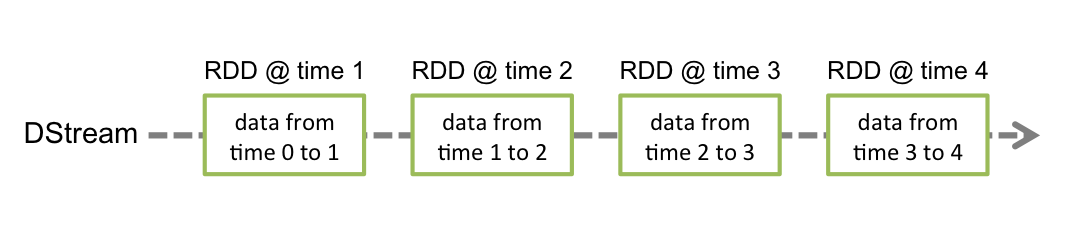
\includegraphics[scale=0.45]{./styles/streaming-dstream.png}
 % streaming-flow.png: 0x0 pixel, 300dpi, 0.00x0.00 cm, bb=
 \caption{DStreams are Spark streaming's abstraction of a data stream}
 \label{fig:dstream}
\end{figure}

